\documentclass[11pt, table, dvipsnames]{beamer}
%\documentclass[11pt,handout]{beamer}
\usepackage{xcolor}
\usepackage[all]{xy}

%\mode<beamer>{% 
%\usetheme[showothersubsections,right,width=17mm]{Goettingen}} 
%\usecolortheme{dove}
%\usecolortheme{lily}

%\mode<beamer>{\usetheme{Boadilla}}

\usepackage{hyperref}
 \title[Retrieving and Parsing Linguistic Expressions of Political Attitudes]{Retrieving and Parsing Linguistic Expressions of Political Attitudes}
\author{Paul Nulty}
\institute % (optional)
{
  Department of Methodology, \\
  London School of Economics and Political Science, \\
  \vspace{2 mm}
  \textit{QUANTESS} ERC Project 
}
 
\date % (optional)
{Computational Social Science, ECCS 2014 \\ 
24th September 2014}


\graphicspath{ {./graphics/} }
\definecolor{customBlue}{rgb}{0.9,0.9,0.95}
\begin{document}

\begin{frame}%<handout:0>
\titlepage
\end{frame}


\begin{frame}
  \frametitle{Social information modes on online networks}
 \begin{itemize}
  \item Network structure (friend, follower, subscriber)
  \item Simple actions: like, retweet, mention, favorite
  \item Multimedia: links, animations, videos, images
  \item Linguistic (text): Posts, comments, tweets
  \end{itemize}
\end{frame}

\begin{frame}
  \frametitle{Linguistic communication}
  \begin{itemize}
  \item Social media offers large, real-time broadcast text corpus of spontaneous communication and expression
  \item Retrieval depends on bursty and ambiguous search terms
  \item NLP offers methods to discover structure and help retrieval
  \end{itemize}
\end{frame}

\begin{frame}
  \frametitle{Natural language on twitter}
  \begin{itemize}
  \item twitter language is non-standard, but can be normalized \footnote{Syntactic normalization of twitter messages, Kaufman and Kalita 2010)}
  \item Simple statistical linguistics can aid retrieval
  \item Syntactic structure of statements can be extracted
  \item Applications: twitter as sensor for public health, natural disasters, sentiment
  \end{itemize}
\end{frame}


\begin{frame}
  \frametitle{Zipf's laws}
  \begin{itemize}
  \item In natural languages, word frequencies have a very heavy-tailed distribution
  \item Zipf's Law (1935): The frequency of a word is inversely proportional to its rank in the frequency table
  \item Zipf (1945): The more frequent a word is, the more senses it is likely to have
  \item frequent search terms give high recall, but low precision
  \end{itemize}
\end{frame}


\begin{frame}
  \frametitle{Rank frequency of terms}
    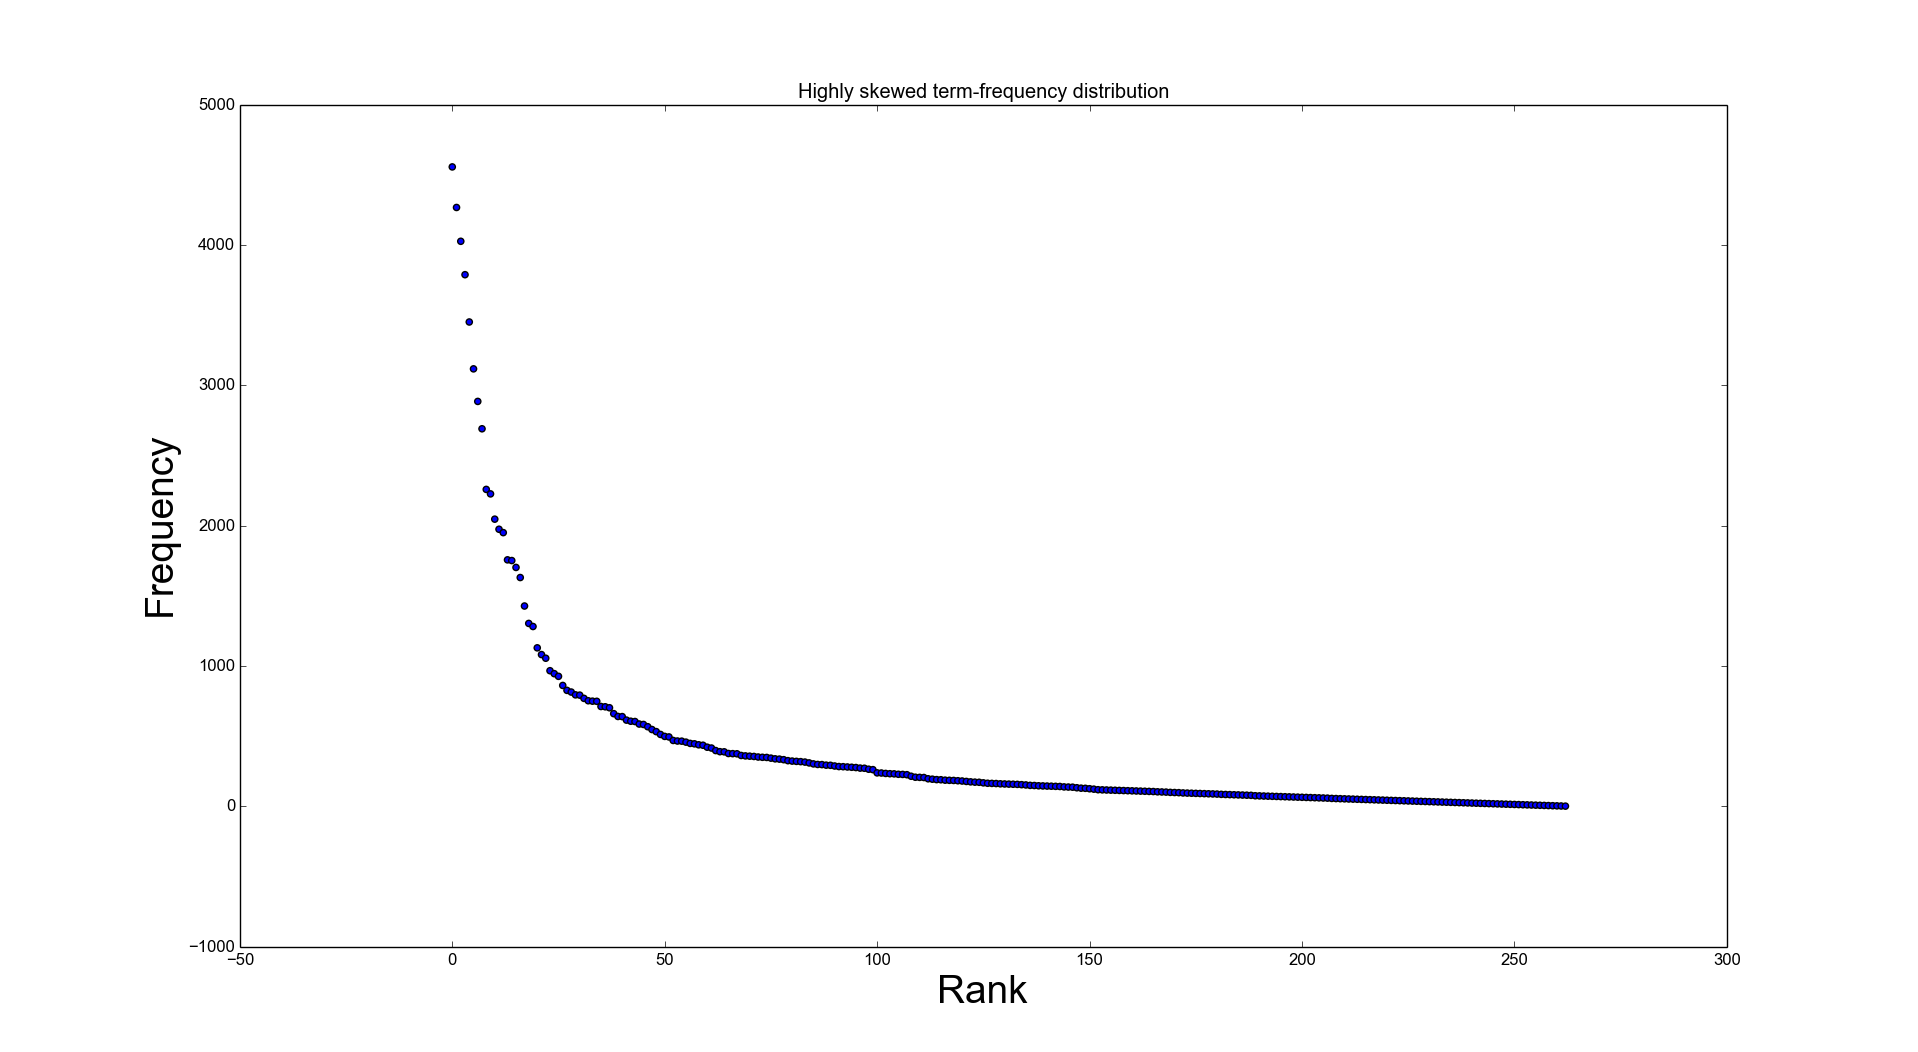
\includegraphics[scale=0.20]{zipf1}\\
  \scriptsize
From 260,619 tweets (no retweets), from twitter `gardenhose' api on Scottish referendum day, containing any of these terms: \texttt{["\#indyref", "salmond", "cameron", "scotland", "scottish", "referendum", "vote", "voted", "voting"]}
\end{frame}

\begin{frame}
  \frametitle{Log-Log Rank frequency}

    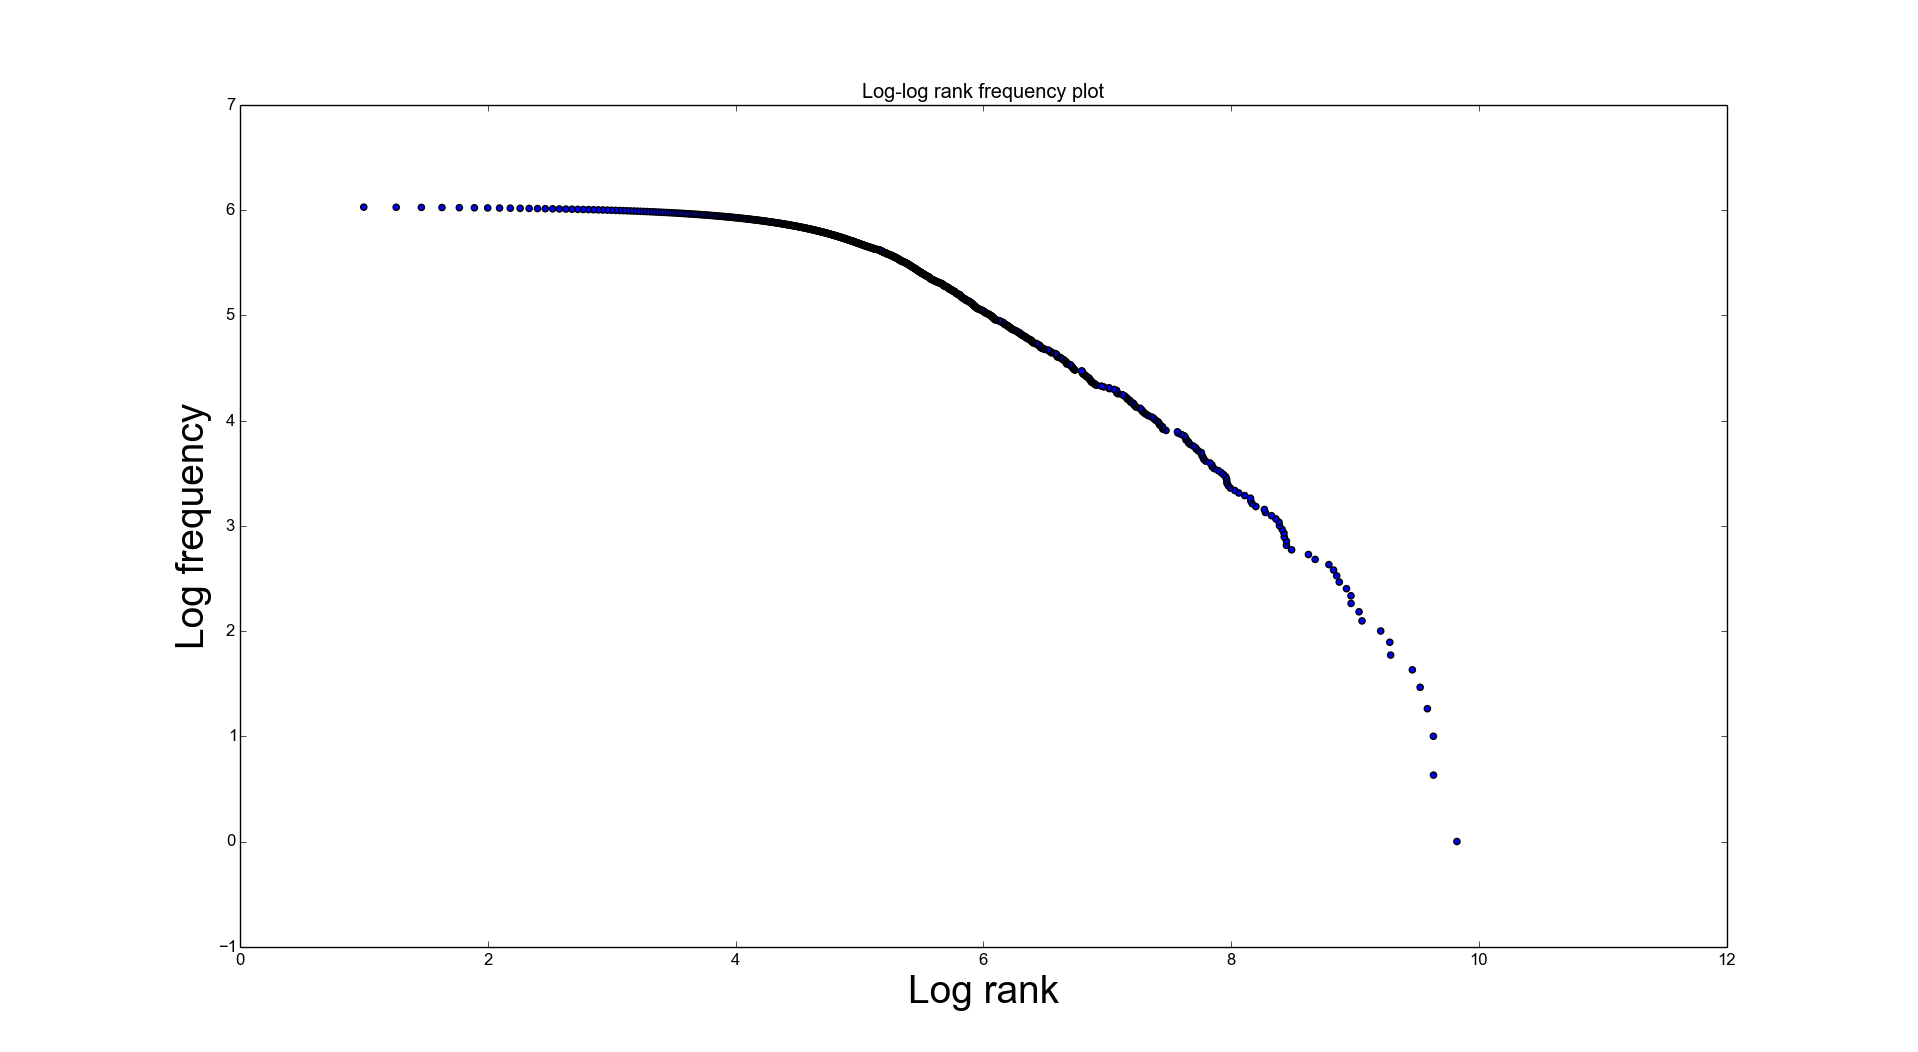
\includegraphics[scale=0.20]{zipf2}\\
  \scriptsize
From 260,619 tweets (excluding retweets, 1.02M total), from twitter `gardenhose' api on Scottish referendum day, containing any of these terms: \texttt{["\#indyref", "salmond", "cameron", "scotland", "scottish", "referendum", "vote", "voted", "voting"]}
\end{frame}



\begin{frame}
  \frametitle{Precision vs Recall}
  \begin{itemize}
  \item Initially, prefer recall over precision
  \item Hone search terms by learning association between terms and concept of interest
  \item e.g. Initially search for "vote", "cameron", "indyref"
  \item learn which terms co-occur with precise concept of interest
  \end{itemize}
\end{frame}

\begin{frame}
  \frametitle{Example: Naive Bayes classifier for Scottish referndum opinion} 
  \begin{itemize}
  \item Treat \#bettertogether and \#voteyes as training labels 
  \item Simple bag-of-words model (without hashtag labels, 800 most common terms)
  \item   \item predicted 1866 out of 2367 tweets correctly (79\%) (out of sample)
  \item Most informative features identify useful terms for further search.
  \end{itemize}
\end{frame}


\begin{frame}
\frametitle{terms predictive of 'no'(\#bettertogether and \#nothanks)}
  \begin{table}[!htbp]\centering
  \rowcolors{1}{customBlue}{White}
\begin{tabular}{p{4cm}p{1.5cm}p{3cm}}
 \hline
term & Direction & Ratio \\
\hline
kingdom        &         no   &    20.7 : 1.0 \\
stupid         &       no    &     16.1 : 1.0 \\
united          &       no    &     15.0 : 1.0 \\
stay           &     no    &      8.9 : 1.0 \\
\#no 		&    no    &       8.6 : 1.0 \\
\#uk		&    no    &      6.6 : 1.0 \\
\#votenoscotland &   no &     6.1 : 1.0 \\
\#voteno 	&    no &        5.5 : 1.0\\
union &               no     &      5.2 : 1.0\\
sense &                 no    &      4.8 : 1.0\\
enough &                no    &      4.8 : 1.0\\
uk &                 no      &      4.4 : 1.0\\
britain &                 no    &      4.3 : 1.0\\
leave &                 no    &      4.3 : 1.0\\
\hline
\end{tabular}
\end{table}
\end{frame}


\begin{frame}
\frametitle{terms predictive of 'yes'(\#voteyes and \#yesscotland)}
\begin{table}[!htbp]\centering
\rowcolors{1}{customBlue}{White}
\begin{tabular}{p{5cm}p{1.5cm}p{3cm}}
\hline
term & Direction & Ratio \\
\hline
\#freedom &                yes      &     29.8 : 1.0\\
\#letsdothis &                yes      &     20.9 : 1.0  \\            
\#voteaye &                yes      &     20.2 : 1.0\\
\#savvy &                yes      &     18.0 : 1.0\\
imagine &                yes     &      9.8 : 1.0\\
opportunity &                yes     &      9.4 : 1.0\\
fairer &                yes     &      9.2 : 1.0\\
\#hopeoverfear &                yes      &      8.1 : 1.0\\
hands &                yes     &      7.6 : 1.0\\
society &                yes     &      7.0 : 1.0\\
\#independence &                yes     &      6.7 : 1.0\\
excited &                yes     &      6.3 : 1.0\\
atsymb\_nicolasturgeon &                yes     &      5.9 : 1.0\\
brave &                yes     &      5.5 : 1.0\\
\hline
\end{tabular}
\end{table}
\end{frame}


\begin{frame}
  \frametitle{Structured Natural language processing}
  \begin{itemize}
  \item Recent methods in NLP have moved beyond bag-of-words model
  \item Named entity recognition, co-reference resolution, 
  \item Typed dependency parsing
  \item Detect specific expressions rather than term mentions
  \item Stanford Core NLP toolkit \footnote{(Manning et al, ACL 2014)}
  \end{itemize}
\end{frame}

\begin{frame}
  \frametitle{Stanford Core NLP: Named entities}
\includegraphics[scale=0.40]{NER}\\
  \scriptsize
\texttt{`atsymb\_YesScotland But the NHS budget in Scotland is 100\% under Scottish Parliament control so privatisation is not an issue.'}
\end{frame}

\begin{frame}
  \frametitle{Stanford Core NLP: typed dependency parse}
\includegraphics[scale=0.60]{votingDeps}\\
  \scriptsize
\texttt{`voting Yes gives hashsymbScotland a better position in Europe/UK in all cases'}
\end{frame}

\begin{frame}
  \frametitle{Classification with dependency relations as features} 
  \begin{itemize}
  \item Treat \#bettertogether and \#voteyes as training labels 
  \item Without relations involving hashtag labels, 60 most common dependencies)
  \item  76\% accuracy out of sample
  \item Need a much bigger corpus for complex features
  \end{itemize}
\end{frame}

\begin{frame}
  \frametitle{Most informative dependency relations (yes side)} 
\begin{table}[!htbp]\centering
\rowcolors{1}{customBlue}{White}
\begin{tabular}{p{5cm}p{1.5cm}p{3cm}}
\hline
term & Direction & Ratio \\
\hline
       dobj\_make\_history &                yes      &      6.9 : 1.0\\
            dobj\_do\_this &                yes      &      5.6 : 1.0\\
   advmod\_important\_most &                yes      &      5.1 : 1.0\\
           nsubj\_vote\_we &                yes      &      5.1 : 1.0\\
             nsubj\_do\_we &                yes      &      4.5 : 1.0\\
             nsubj\_do\_'s &                yes      &      4.3 : 1.0\\
        nn\_Scotland\_luck &                yes      &      3.9 : 1.0\\
\hline
\end{tabular}
\end{table}

\end{frame}

\begin{frame}
  \frametitle{thank you} 
  \begin{itemize}
  \item Thank you for yoru attention
  \item Code available \texttt{https://github.com/pnulty/oiicss}
  \end{itemize}
\end{frame}





\end{document}
